\chapter{Design} \label{chap:design}

This chapter presents the design of a workstation to reduce impact of phishing attacks. Phishing attacks usually operate by misleading users into trusting malicious content as being genuine. The design includes several policies to be enforced by the browsing client.

\paragraph{Site Aggregate Isolation:} Modern internet applications consist of content from different sources: user-generated content, external APIs, etc. This makes it difficult to identify the source of the content a users sees. Phishing attacks take advantage of this by displaying content that appears to be created by a genuine source. We present a new policy called Site Aggregate Isolation to defend against such attacks. The policy dictates that content from different sources (or \textit{site-aggregates}) must be explicitly displayed in isolated environments.

\paragraph{Cross Site-Aggregate Resources:} Since applications need to display content from different site-aggregates, we describe exceptions to the Site Aggregate Isolation policy for resources to be included from other site-aggregates in a safe way.

\paragraph{External Resource Referrer:} Some attacks operate by stealing information from external websites, for example, by stealing information from internal APIs belonging to third-party websites. We introduce a policy to defend against such unauthorized cross site-aggregate requests.

\paragraph{Exit Destinations:} Modern applications also rely on communication among one another. Phishing attacks take advantage of this by being able to steal information and submitting it to the attacker's server. We present a policy to defend against unauthorized communication between websites.

\paragraph{HTTP Response Headers:} The policies presented in this chapter requires additional information from websites. Websites currently do not provide information about their site-aggregate name, external resources they require, or external URLs they may communicate with. To extract this information from the websites, we introduce four new HTTP response headers: \texttt{Site-Aggregate},  \texttt{Site-Aggregate-Pattern}, \texttt{Cross-Site-Aggregate-Resource-Pattern}, and \texttt{Exit-Pattern}.

\paragraph{DNSSEC and SSL/TLS Certificates:} A popular way phishing attacks operate is by DNS spoofing or DNS cache poisoning. We present policies to prevent against these attacks.

\paragraph{User Interface:} In addition to securing the web browsing backend, we present the design of a secure user interface. Phishing attacks trick the user by taking advantage of the ambiguity of the user interface. We discuss the limitations of the current user interfaces that use stacking window managers. We also present a clear and unambiguous user interface by introducing a single-application window manager inspired by smartphones.

\section{Site Aggregate Isolation} \label{same_origin_isolation}

While browsing, one of the primary concerns of the user is to ensure that the content they see is genuine. One way to approach this would be to forbid all content that was not created by the owner of the website the user intended to visit. However, such a strict policy would be impractical. Modern internet applications rely heavily on content from several sources, for example, user-generated content, external APIs, etc. Additionally, applications such as social networking websites and email are based around user created content. On the other hand, allowing all content, which is what current browsers do, is also not ideal as it is the main reason behind deceptive content being displayed to the user.

A more flexible policy is needed which still preserves the interactivity of websites allowing them to feature user created content, but also making it clear to the user that certain parts of the website are not created by the website owner and making it visually explicit when the user navigates to a content that was not created by the original website that the user visited.

In the design of a secure workstation, we enforce a policy called Site Aggregate Isolation. An \textit{site-aggregate} is defined as a website or a group of website that coherently form a single unit. For example, Bank of America and Reddit are part of different site-aggregates. The decision to come up with this group is up to the website developers. For example, Google may designate Gmail, Search, News, YouTube, etc. as different site-aggregates. The policy states that web applications belonging to different site-aggregates must be completely isolated from each other, both on the backend side and the user interface side. They must not be able to communicate or transfer data with each other unless both websites explicitly agree otherwise. Additionally, web applications belonging to different site-aggregates must be visually separate and display identifying information about the site-aggregate name at all times.

\section{Cross Site-Aggregate Resources}

Site Aggregate Isolation policy can be too strict for the scenario of websites requesting resources from another website. This is commonly seen for Content Delivery Network (CDN) websites where a popular resource such as a Javascript library is hosted by a mass distribution CDN service and third-party websites can then link back to the CDN and request the external resource. This provides several advantages such as the ability cache common libraries for different websites and faster response times for the resources hosted on the CDN. These external resources however must not be considered as being on the same site-aggregate as a third-party website as they are not served by that website itself.

A policy exception needs to be defined for such resources. The cross site-aggregate resource exception to the policy states that if a website requests resources from an external website not in the same site-aggregate, it must:
\begin{itemize}
    \item provide information such as the cryptographic checksums of the resource so that the browser can verify the integrity of the external resource, and
    \item explicitly enlist the address of the resource in a separate cross site-aggregate resource list.
    \item provide a signature for the cross site-aggregate resource list for the browser to verify that the list has not been tampered with
\end{itemize}
%This is because this can lead to a transitive effect where two websites A and B initially on different origins may be mistakenly considered to be on the same origin since they both list the shared resource on the CDN to be their own respective origin.

\section{External Resource Referrer}

The policy and its exception discussed previously provide safety against a website requesting and displaying resources that the website owner didn't intend to include. However, it doesn't prevent third-party websites from defending against unauthorized requests. For example, Site A may try to access content from Site B however Site B may not want to provide the content to Site A, because that content is internal to Site B.

We implement an external resource referrer policy on all cross site-aggregate resource requests. The policy requires all requests to contain the site-aggregate of the website requesting the resource. Web servers must verify the referrer of all incoming requests and deny serving any requests that are unauthorized for that referrer.

\section{Exit Destinations}

Some phishing websites may still be able to embed themselves into another website. For example, they may be able to inject a HTML form into your social networking feed. They may try to trick the user into entering their password in a fake login form. When the user clicks on the button, they may be redirected to an external page belonging to the attacker where the information may be posted. such attacks may be prevented by restricting the possible exit destinations that a web page is allowed to send information to.

To isolate different site-aggregates and preventing them from sending information to each other, no form data must be allowed to be sent to an external site-aggregate either via a GET or a POST request. However, such a strict policy will again not be able to support modern web applications which may want to submit data elsewhere. To support this, the website must explicitly list all exit URLs in an exit destination list. The website must also provide a signature for this list. The browser must verify the signature and only allow information to be posted if the external URL matches one of the URLs in the exit destination list.

\section{HTTP Response Headers}

The policies introduced in the previous sections require additional information from websites such as their site-aggregate names, list of external resources, etc. We use HTTP response headers to extract this information. In this section, we introduce new HTTP response headers that websites must include to support the system.

\subsection{\texttt{Site-Aggregate-Name}}

Every page must have the {\tt Site-Aggregate-Name} header field which contains the name of the site-aggregate that page belongs to. For example all webpages from {\tt facebook.com} and {\tt fb.com} may have the value of the {\tt Site-Aggregate-Name} header field to be {\tt facebook.com}, since both the domains names are used by Facebook and are part of a single unit. It must be ensured that these names are web-requestable URLs. This is used in verification of the site-aggregate name as explained in future sections.

\subsection{\texttt{Site-Aggregate-Pattern}}

The {\tt Site-Aggregate-Pattern} header field is included in the HTTP response of every web page. This field must include the URL patterns in the form of regular expressions for all the URLs that are considered part of the same site-aggregate as the requested web page. There may be multiple {\tt Site-Aggregate-Pattern} headers in the response which may list additional URLs to be considered part of the same site-aggregate. The filter considers the union of all the site-aggregate patterns to decide if a requested web page is in the same site-aggregate or not.

For example, responses from Gmail may include the following {\tt Site-Aggregate-Pattern} header fields:

\begin{verbatim}
Site-Aggregate-Pattern: https:\/\/mail.google.com\/.*
Site-Aggregate-Pattern: https?:\/\/(www\.)?gmail.com\/.*
Site-Aggregate-Pattern: https:\/\/accounts\.google\.com\/signin\/gmail\/.*
\end{verbatim}

Since multiple instances of the header field are converted to a union, these pattern match any webpages which begin with {\tt gmail.com} or {\tt mail.google.com} domains or are the sign-in pages at {\tt accounts.google.com/signin/gmail}. This ensures that even if any malicious content shows up within these pages, it won't be able to redirect the user to fake login pages outside the Gmail's list of allowed URL's.

\subsection{\texttt{Cross-Site-Aggregate-Resource-Pattern}}

Most webpages include resources from external sources. These may include Javascript from a CDN, external images or even HTML IFrames. To allow these resources to be loaded, we introduce the {\tt Cross-Site-Aggregate-Resource-Pattern} header field. This field lists the URL patterns of all external resources that the webpage requires in the form of regular expressions. The proxy filter allows requests to these URLs given that the request originates in form of an external resource request from the browser and not as a standalone request. The request gets blocked if the user attempts to directly navigate to these resources.

For example, a website which includes JQuery, a Javascript framework, and Google Fonts may have the following {\tt Cross-Site-Aggregate-Resource-Pattern} header fields:

\begin{verbatim}
Cross-Site-Aggregate-Resource-Pattern: https:\/\/fonts\.googleapis\.com
                                       \/css\/Roboto
Cross-Site-Aggregate-Resource-Pattern: https?:\/\/code\.jquery\.com
                                       \/jquery-3\.2\.1\.slim\.min\.js
\end{verbatim}

These headers ensure that the webpage can load these resources even though they belong to a different site-aggregate. Restricting direct navigation to these URLs also ensures that these resources can't disguise themselves as Javascript and in reality serve as full HTML page.

\subsection{\texttt{Exit-Pattern}}

It is possible for webpages to include direct HTML content from an external source. For example, HTML emails or external advertisements. In the event this external source gets compromised, it can serve malicious content to the user. A common form of exploitation technique is to present a fake login form to the user in the space that was meant only for advertisements. This can trick the user into entering their credentials and submitting it to a URL of different site-aggregate. To prevent this attack, we introduce the {\tt Exit-Pattern} header field. This field lists the allowed URLs of different site-aggregates which the user is allowed to post any information to. For all other URLs, any information posted in the form of GET or POST parameters is prohibited. The user is always allowed to post information to URLs within the same site-aggregate.

For example, the website LMGTFY allows users to search for content from various search engines. This website can include the following list in its response headers:

\begin{verbatim}
Exit-Pattern: https?:\/\/www\.google\.com\/q\/.*
Exit-Pattern: https?:\/\/www\.bing\.com\/search.*
Exit-Pattern: https?:\/\/search\.aol\.com\/aol\/search.*
\end{verbatim}

This will allow LMGTFY to post search queries to these external URLs only, and thus prevent any information to be posted by mistake to any other potentially malicious URL.

\section{DNSSEC and SSL/TLS Certificates}

DNS spoofing or DNS cache poisoning is a popular way phishing attacks work. The attacker can corrupt the DNS cache of the user's system or can even act as a DNS proxy for the user. The attacker can then modify the DNS entries for websites and point them to the his/her version of the website to steal user credentials. For example, the attacker may spoof DNS entries for {\tt facebook.com} and redirect it to display a fake login page for Facebook. The attacker can then steal the credentials and redirects the user to the real Facebook login page to avoid suspicion.

A technology called DNSSEC can be used to prevent such attacks. DNSSEC is an extension to the Domain Name System which allows DNS entries to be cryptographically signed. It provides a chain of trust that can be verified all the way to the root nameservers. If an attacker is able to modify the DNS responses, he/she will not be able to provide a signature for the new responses since the signing key is not public. However, a lot of websites still haven't implemented this system. We strongly recommend the implementation of DNSSEC to secure DNS entries.

A related attack method would be for the attacker to act as a proxy. The attacker can then analyze and modify all traffic and be able to steal credentials or trick the user into downloading malicious software. However nowadays, most websites use end to end encryption using SSL/TLS certificates. These certificates are distributed by organizations called Certificate Authorities (CAs). The CA issues these certificates only to the owner of the websites. The browser can verify that the domain in the certificate matches the actual domain of the website. However, the CAs may make a mistake when verifying website ownership and may give certificates to malicious third-parties too \cite{chinese-ca}.

Such attacks can be prevented using DNS-based Authentication of Named Entities (DANE). The DANE protocol specifies putting the public keys of the SSL/TLS certificates of websites in DNS entries themselves. With DNSSEC in place to sign the DANE entries, the browsers can verify that the web server they are talking to using end to end encryption is correct and no attacker has spoofed the certificates.

The secure workstation must have the capability to perform DNSSEC and DANE verifications. If these checks fail, it must notify the user that the request was denied due to such a failure.

\section{User Interface} \label{userinterface}

The user interface is the main target of several phishing attacks. Most attacks try to mimic the system UI and trick the user into clicking and downloading malicious content. For example, a phishing page might display that the user's computer has a virus and that they must click on a link to download an antivirus software. However, the antivirus software turns out to be a malicious software which can compromise the user's system.

\begin{figure}[p]
\centering
    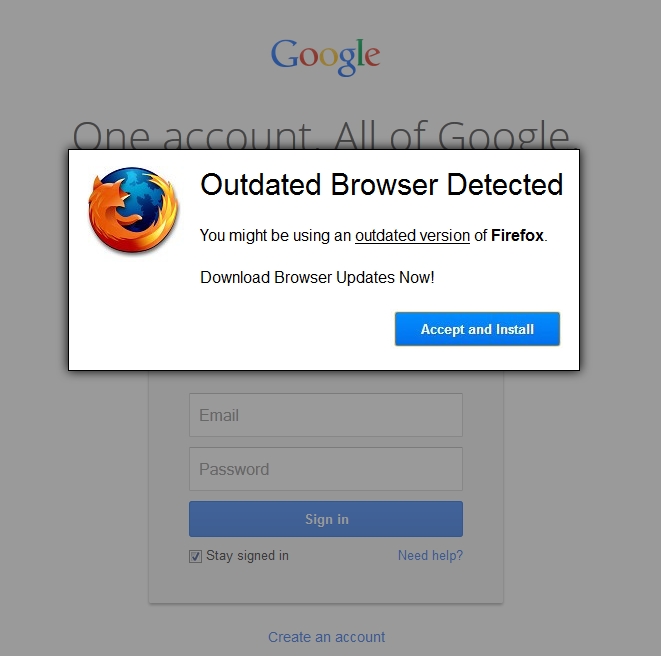
\includegraphics[width=1.0\textwidth]{ff2.png}
    \caption{This figure shows a phishing page which is prompting the user to update their browser by clicking on the link.}
   \label{fig:fakeprompt-1}
\end{figure}
\begin{figure}[p]
\centering
    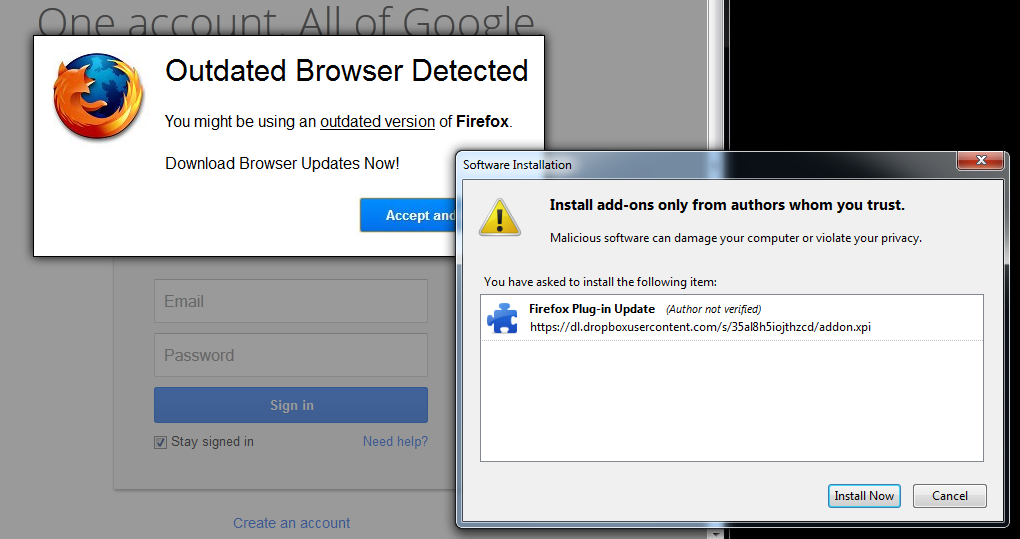
\includegraphics[width=1.0\textwidth]{ff-addon1.png}
    \caption{This figure shows the same phishing page as before after the user clicks on the link. The links leads to the browser installing a malicious add-on disguised as a fake update.}
   \label{fig:fakeprompt-2}
\end{figure}

This is made possible largely due to the use of stacking window managers in modern day systems. A stacking window manager lets the user resize, move and arrange windows in any way they want. This leads to ambiguity between which window belongs to the website and which window belongs to the system.

Figures \ref{fig:fakeprompt-1} and \ref{fig:fakeprompt-2} show an example of a phishing page which tricks the user into believing that Firefox is need of an update. When the user clicks on the update link, the browser downloads a malicious add-on. The add-on is disguised to appear as a Firefox update.

The user interface for the secure workstation must be free of such disambiguities. Taking inspiration from user interfaces of smart phones, we propose the user interface to be a single application window manager. Only one website can be displayed on the screen at any time. This is in contrast to how stacking window managers work with multiple applications overlapping each other. A single application interface will only display one application which occupies the entire screen space. In addition, there should be some screen space reserved for system prompts and notifications. Applications shouldn't be able to modify and display anything in this reserved space. Vice-versa, system prompts and notifications should never appear in the application area. This will make sure if a user sees anything in the reserved area they can trust that it is shown by the system and not by some application pretending to be the system.

Additionally, the user interface must also display the site-aggregate name and the URL of the current webpage at all times. This information should be visible in the reserved area and not writable by the websites themselves. Apart from the site-aggregate name, the user interface can also display the name of the organization or website to the user. This information can be obtained from the SSL/TLS certificates of the website.

The user may choose to mark specific websites as known and trusted. For example, the user may visit their banking website and mark it as trusted. The user interface must show visual indication whenever the user visits a trusted website. This will be helpful in case a phishing website is able to display the bank login page. The user can verify that the phishing webpage is not trusted since it does not have a trusted visual indication.
